% DIALS architecture. Build: pdflatex architecture.tex && pdftoppm -png -r 220 -singlefile architecture.pdf architecture
\documentclass[tikz,border=8pt]{standalone}
\usepackage{amsmath,amssymb}
\usepackage{fontawesome5}
\usetikzlibrary{arrows.meta,calc}
\definecolor{fzfill}{HTML}{E3EFFA}\definecolor{fzline}{HTML}{3B7FC4}
\definecolor{trfill}{HTML}{FDE6CF}\definecolor{trline}{HTML}{D9730D}
\definecolor{cC}{HTML}{7B4FB8}\definecolor{cL}{HTML}{1C9A8A}\definecolor{cG}{HTML}{3A8F3A}\definecolor{cS}{HTML}{C8372D}
\newcommand{\fire}{{\color{trline}\faFire}}
\newcommand{\snow}{{\color{fzline}\faSnowflake}}
\tikzset{
  arr/.style={-{Stealth[length=2.4mm]},line width=0.7pt,draw=black!70},
  bus/.style={line width=0.9pt,draw=black!70},
  frozen/.style={draw=fzline,fill=fzfill,line width=0.8pt,rounded corners=1.5pt},
  train/.style={draw=trline,fill=trfill,line width=0.9pt,rounded corners=3pt},
  tower/.style={draw=black!35,fill=black!2,line width=0.8pt,rounded corners=8pt},
  lab/.style={font=\small},
  tiny/.style={font=\scriptsize},
  op/.style={circle,draw=black!70,line width=0.8pt,minimum size=6mm,inner sep=0pt,fill=white},
}
% a horizontal score vector over the catalogue, one shaded cell per item: centre x, y, colour
\newcommand{\scorebar}[3]{%
  \foreach \v [count=\i] in {25,70,15,85,40,55,10,95,35,20,65,45}{
    \fill[#3!\v!white] ($(#1,#2)+({(\i-7)*0.24},0)$) rectangle ++(0.24,0.32);}
  \draw[black!60,line width=0.5pt] ($(#1,#2)+(-1.44,0)$) rectangle ++(2.88,0.32);}
\newcommand{\mat}[5]{\draw[#5] (#1,#2) rectangle ++(#3,#4);}  % x, y, width, height, style

\begin{document}
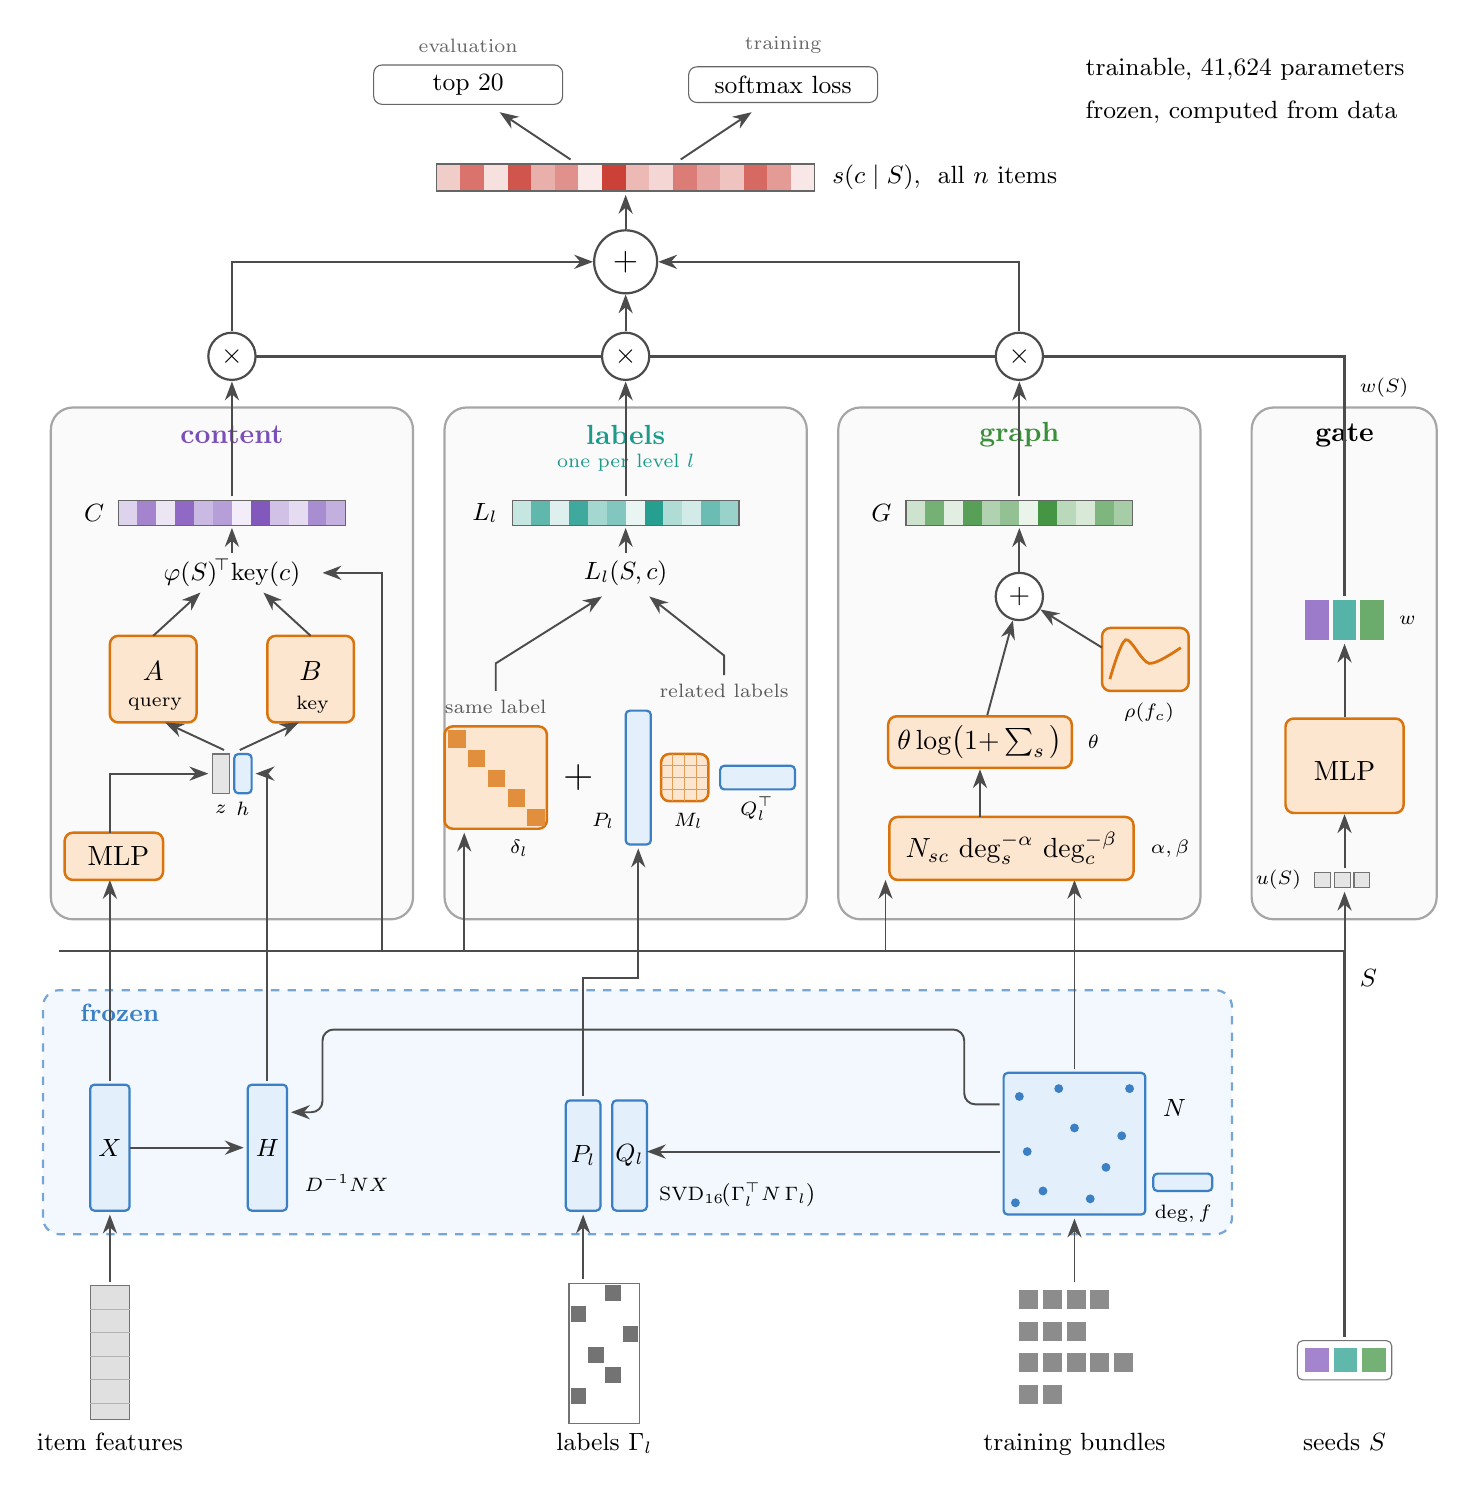
\begin{tikzpicture}[x=1cm,y=1cm]

% ============================================================ INPUTS (bottom)
\fill[black!12] (0.9,0) rectangle ++(0.5,1.7);\draw[black!55] (0.9,0) rectangle ++(0.5,1.7);
\foreach \y in {0.2,0.5,...,1.5}{\draw[black!30] (0.9,\y) -- ++(0.5,0);}
\node[lab,below] at (1.15,-0.05) {item features};
\foreach \r/\c in {0/2,1/0,2/3,3/1,4/2,5/0}{\fill[black!55] (7.0+0.22*\c,1.5-0.26*\r) rectangle ++(0.2,0.2);}
\draw[black!55] (6.98,-0.05) rectangle (7.88,1.72);
\node[lab,below] at (7.43,-0.05) {labels $\Gamma_l$};
\foreach \row/\len in {0/4,1/3,2/5,3/2}{\foreach \k in {1,...,\len}{\fill[black!45] (12.4+0.3*\k,1.4-0.4*\row) rectangle ++(0.24,0.24);}}
\node[lab,below] at (13.4,-0.05) {training bundles};
\foreach \k/\c in {0/cC,1/cL,2/cG}{\fill[\c!70] (16.33+0.36*\k,0.6) rectangle ++(0.3,0.3);}
\draw[black!55,rounded corners=2pt] (16.23,0.5) rectangle (17.43,1.0);
\node[lab,below] at (16.83,-0.05) {seeds $S$};

% ============================================================ FROZEN DATA
\draw[fzline!70,dashed,fill=fzfill!45,rounded corners=6pt,line width=0.8pt] (0.3,2.35) rectangle (15.4,5.45);
\node[anchor=north west,font=\small\bfseries,text=fzline] at (0.4,5.4) {\snow\ \ frozen};
% X, H
\mat{0.9}{2.65}{0.5}{1.6}{frozen}\node[lab] at (1.15,3.45) {$X$};
\mat{2.9}{2.65}{0.5}{1.6}{frozen}\node[lab] at (3.15,3.45) {$H$};
\node[tiny,anchor=west] at (3.5,3.0) {$D^{-1}NX$};
\draw[arr] (1.4,3.45) -- (2.85,3.45);
% P, Q
\mat{6.94}{2.65}{0.44}{1.4}{frozen}\mat{7.53}{2.65}{0.44}{1.4}{frozen}
\node[lab] at (7.16,3.35) {$P_l$};\node[lab] at (7.75,3.35) {$Q_l$};
\node[tiny,anchor=west] at (8.0,2.85) {SVD$_{16}\!\big(\Gamma_l^{\top} N\, \Gamma_l\big)$};
% N, deg, f
\mat{12.5}{2.6}{1.8}{1.8}{frozen}
\foreach \x/\y in {0.2/1.5,0.5/0.3,0.9/1.1,1.3/0.6,0.3/0.8,1.6/1.6,1.1/0.2,0.7/1.6,1.5/1.0,0.15/0.15}{\fill[fzline] (12.5+\x,2.6+\y) circle (1.6pt);}
\node[lab,anchor=west] at (14.4,3.95) {$N$};
\mat{14.4}{2.9}{0.75}{0.22}{frozen}\node[tiny,anchor=north] at (14.78,2.85) {$\deg, f$};
% how they are built
\draw[arr] (1.15,1.75) -- (1.15,2.6);
\draw[arr] (7.16,1.78) -- (7.16,2.6);
\draw[arr] (13.4,1.75) -- (13.4,2.55);
\draw[arr] (12.45,3.4) -- (7.97,3.4);
\draw[arr,rounded corners=4pt] (12.45,4.0) -- (12.0,4.0) -- (12.0,4.95) -- (3.85,4.95) -- (3.85,3.9) -- (3.45,3.9);

% ============================================================ SEED BUS
\draw[bus] (16.83,1.05) -- (16.83,5.95) -- (0.5,5.95);
\node[lab,anchor=west] at (16.9,5.6) {$S$};

% ============================================================ TOWERS
\foreach \x/\c/\t in {2.7/cC/content,7.7/cL/labels,12.7/cG/graph}{
  \draw[tower] (\x-2.3,6.35) rectangle (\x+2.3,12.85);
  \node[font=\bfseries,text=\c] at (\x,12.5) {\t};}
\node[tiny,text=cL] at (7.7,12.15) {one per level $l$};
\draw[tower] (15.65,6.35) rectangle (18.0,12.85);\node[font=\bfseries] at (16.83,12.5) {gate};

% ---------------- content
\draw[arr] (1.15,4.3) -- (1.15,6.85);                       % X
\draw[arr] (3.15,4.3) -- (3.15,8.2) -- (3.0,8.2);           % H
\draw[arr] (4.6,5.95) -- (4.6,10.75) -- (3.85,10.75);       % S
\node[train,minimum width=1.25cm,minimum height=0.6cm] (mlp) at (1.2,7.15) {\fire\ MLP};
\draw[black!55,fill=black!10] (2.45,7.95) rectangle ++(0.22,0.5);\draw[frozen] (2.73,7.95) rectangle ++(0.22,0.5);
\node[tiny] at (2.56,7.75) {$z$};\node[tiny] at (2.84,7.75) {$h$};
\draw[arr] (1.15,7.45) -- (1.15,8.2) -- (2.4,8.2);
\draw[train] (1.15,8.85) rectangle ++(1.1,1.1);\draw[train] (3.15,8.85) rectangle ++(1.1,1.1);
\node at (1.7,9.5) {$A$};\node at (3.7,9.5) {$B$};
\node[tiny] at (1.7,9.08) {\fire\,query};\node[tiny] at (3.7,9.08) {\fire\,key};
\draw[arr] (2.6,8.5) -- (1.85,8.85);\draw[arr] (2.8,8.5) -- (3.55,8.85);
\node[lab] (cf) at (2.7,10.75) {$\varphi(S)^{\!\top}\mathrm{key}(c)$};
\draw[arr] (1.7,9.95) -- (2.3,10.5);\draw[arr] (3.7,9.95) -- (3.1,10.5);
\scorebar{2.7}{11.35}{cC}\node[lab,anchor=east] at (1.2,11.51) {$C$};
\draw[arr] (2.7,11.0) -- (2.7,11.32);

% ---------------- labels: diagonal + low rank
\draw[arr] (5.65,5.95) -- (5.65,7.45);                      % S
\draw[arr] (7.16,4.1) -- (7.16,5.6) -- (7.86,5.6) -- (7.86,7.25);   % P, Q
\draw[train] (5.4,7.5) rectangle ++(1.3,1.3);
\foreach \k in {0,...,4}{\fill[trline!80] (5.45+0.25*\k,8.53-0.25*\k) rectangle ++(0.22,0.22);}
\node[tiny] at (6.3,7.25) {\fire\ $\delta_l$};
\node[font=\Large] at (7.1,8.15) {$+$};
\mat{7.7}{7.3}{0.32}{1.7}{frozen}
\draw[train] (8.15,7.85) rectangle ++(0.6,0.6);
\foreach \k in {0.15,0.3,0.45}{\draw[trline!70,line width=0.4pt] (8.15+\k,7.85) -- ++(0,0.6);\draw[trline!70,line width=0.4pt] (8.15,7.85+\k) -- ++(0.6,0);}
\mat{8.9}{8.0}{0.95}{0.3}{frozen}
\node[tiny,anchor=east] at (7.68,7.6) {$P_l$};\node[tiny] at (8.45,7.6) {\fire\ $M_l$};\node[tiny] at (9.37,7.75) {$Q_l^{\top}$};
\node[tiny,text=black!65] at (6.05,9.05) {same label};\node[tiny,text=black!65] at (8.95,9.25) {related labels};
\draw[arr] (6.05,9.25) -- (6.05,9.6) -- (7.4,10.45);
\draw[arr] (8.95,9.45) -- (8.95,9.7) -- (8.0,10.45);
\node[lab] at (7.7,10.75) {$L_l(S,c)$};
\scorebar{7.7}{11.35}{cL}\node[lab,anchor=east] at (6.2,11.51) {$L_l$};
\draw[arr] (7.7,11.0) -- (7.7,11.32);

% ---------------- graph
\draw[arr] (11.0,5.95) -- (11.0,6.85);                      % S
\draw[arr] (13.4,4.45) -- (13.4,6.85);                      % N
\node[train,minimum width=3.1cm,minimum height=0.8cm] (deg) at (12.6,7.25) {$N_{sc}\,\deg_s^{-\alpha}\,\deg_c^{-\beta}$};
\node[tiny,anchor=west] at (14.2,7.25) {\fire\,$\alpha,\beta$};
\node[train,minimum width=2.3cm,minimum height=0.65cm] (damp) at (12.2,8.6) {$\theta\log\!\big(1{+}\textstyle\sum_s\big)$};
\node[tiny,anchor=west] at (13.4,8.6) {\fire\,$\theta$};
\draw[arr] (12.2,7.65) -- (damp);
\draw[train] (13.75,9.25) rectangle ++(1.1,0.8);
\draw[trline,line width=1pt] plot[smooth] coordinates {(13.85,9.4) (14.05,9.9) (14.35,9.6) (14.75,9.8)};
\node[tiny,anchor=north] at (14.3,9.22) {\fire\ $\rho(f_c)$};
\node[op] (gplus) at (12.7,10.45) {$+$};
\draw[arr] (damp) -- (gplus);\draw[arr] (13.75,9.8) -- (gplus);
\scorebar{12.7}{11.35}{cG}\node[lab,anchor=east] at (11.2,11.51) {$G$};
\draw[arr] (gplus) -- (12.7,11.32);

% ---------------- gate
\foreach \k in {0,1,2}{\draw[black!55,fill=black!10] (16.45+0.25*\k,6.75) rectangle ++(0.2,0.2);}
\node[tiny,anchor=east] at (16.4,6.85) {$u(S)$};
\draw[arr] (16.83,5.95) -- (16.83,6.7);
\node[train,minimum width=1.5cm,minimum height=1.2cm,align=center] (gmlp) at (16.83,8.3) {\fire\\[-1pt]MLP};
\draw[arr] (16.83,7.0) -- (gmlp);
\foreach \k/\c in {0/cC,1/cL,2/cG}{\fill[\c!75] (16.33+0.35*\k,9.9) rectangle ++(0.3,0.5);}
\node[tiny,anchor=west] at (17.4,10.15) {$w$};
\draw[arr] (gmlp) -- (16.83,9.85);

% ============================================================ WEIGHTED SUM
\draw[bus] (16.83,10.45) -- (16.83,13.5) -- (2.7,13.5);
\node[tiny,anchor=west] at (16.9,13.1) {$w(S)$};
\foreach \x in {2.7,7.7,12.7}{\node[op] at (\x,13.5) {$\times$};\draw[arr] (\x,11.72) -- (\x,13.18);}
\node[op,minimum size=8mm,font=\large] (sum) at (7.7,14.7) {$+$};
\draw[arr] (2.7,13.82) -- (2.7,14.7) -- (sum);\draw[arr] (7.7,13.82) -- (sum);\draw[arr] (12.7,13.82) -- (12.7,14.7) -- (sum);

% ============================================================ SCORE AND OUTPUT
\begin{scope}
\foreach \v [count=\i] in {25,70,15,85,40,55,10,95,35,20,65,45,30,75,50,12}{\fill[cS!\v!white] ({5.3+(\i-1)*0.3},15.6) rectangle ++(0.3,0.34);}
\draw[black!60,line width=0.5pt] (5.3,15.6) rectangle ++(4.8,0.34);
\end{scope}
\node[lab,anchor=west] at (10.2,15.77) {$s(c\mid S)$, \ all $n$ items};
\draw[arr] (sum) -- (7.7,15.55);
\draw[arr] (7.0,16.0) -- (6.1,16.6);\draw[arr] (8.4,16.0) -- (9.3,16.6);
\node[draw=black!60,rounded corners=3pt,lab,minimum width=2.4cm] at (5.7,16.95) {top 20};
\node[draw=black!60,rounded corners=3pt,lab,minimum width=2.4cm] at (9.7,16.95) {softmax loss};
\node[tiny,text=black!60] at (5.7,17.45) {evaluation};\node[tiny,text=black!60] at (9.7,17.45) {training};

% ============================================================ LEGEND
\node[anchor=west,lab] at (13.2,17.15) {\fire\ \ trainable, 41{,}624 parameters};
\node[anchor=west,lab] at (13.2,16.6) {\snow\ \ frozen, computed from data};
\end{tikzpicture}
\end{document}
